\documentclass[twoside]{book}

% Packages required by doxygen
\usepackage{fixltx2e}
\usepackage{calc}
\usepackage{doxygen}
\usepackage{graphicx}
\usepackage[utf8]{inputenc}
\usepackage{makeidx}
\usepackage{multicol}
\usepackage{multirow}
\PassOptionsToPackage{warn}{textcomp}
\usepackage{textcomp}
\usepackage[nointegrals]{wasysym}
\usepackage[table]{xcolor}

% Font selection
\usepackage[T1]{fontenc}
\usepackage{mathptmx}
\usepackage[scaled=.90]{helvet}
\usepackage{courier}
\usepackage{amssymb}
\usepackage{sectsty}
\renewcommand{\familydefault}{\sfdefault}
\allsectionsfont{%
  \fontseries{bc}\selectfont%
  \color{darkgray}%
}
\renewcommand{\DoxyLabelFont}{%
  \fontseries{bc}\selectfont%
  \color{darkgray}%
}
\newcommand{\+}{\discretionary{\mbox{\scriptsize$\hookleftarrow$}}{}{}}

% Page & text layout
\usepackage{geometry}
\geometry{%
  a4paper,%
  top=2.5cm,%
  bottom=2.5cm,%
  left=2.5cm,%
  right=2.5cm%
}
\tolerance=750
\hfuzz=15pt
\hbadness=750
\setlength{\emergencystretch}{15pt}
\setlength{\parindent}{0cm}
\setlength{\parskip}{0.2cm}
\makeatletter
\renewcommand{\paragraph}{%
  \@startsection{paragraph}{4}{0ex}{-1.0ex}{1.0ex}{%
    \normalfont\normalsize\bfseries\SS@parafont%
  }%
}
\renewcommand{\subparagraph}{%
  \@startsection{subparagraph}{5}{0ex}{-1.0ex}{1.0ex}{%
    \normalfont\normalsize\bfseries\SS@subparafont%
  }%
}
\makeatother

% Headers & footers
\usepackage{fancyhdr}
\pagestyle{fancyplain}
\fancyhead[LE]{\fancyplain{}{\bfseries\thepage}}
\fancyhead[CE]{\fancyplain{}{}}
\fancyhead[RE]{\fancyplain{}{\bfseries\leftmark}}
\fancyhead[LO]{\fancyplain{}{\bfseries\rightmark}}
\fancyhead[CO]{\fancyplain{}{}}
\fancyhead[RO]{\fancyplain{}{\bfseries\thepage}}
\fancyfoot[LE]{\fancyplain{}{}}
\fancyfoot[CE]{\fancyplain{}{}}
\fancyfoot[RE]{\fancyplain{}{\bfseries\scriptsize Generated on Sat Jan 14 2017 17\+:19\+:59 for X\+M\+Leru\+Handleru by Doxygen }}
\fancyfoot[LO]{\fancyplain{}{\bfseries\scriptsize Generated on Sat Jan 14 2017 17\+:19\+:59 for X\+M\+Leru\+Handleru by Doxygen }}
\fancyfoot[CO]{\fancyplain{}{}}
\fancyfoot[RO]{\fancyplain{}{}}
\renewcommand{\footrulewidth}{0.4pt}
\renewcommand{\chaptermark}[1]{%
  \markboth{#1}{}%
}
\renewcommand{\sectionmark}[1]{%
  \markright{\thesection\ #1}%
}

% Indices & bibliography
\usepackage{natbib}
\usepackage[titles]{tocloft}
\setcounter{tocdepth}{3}
\setcounter{secnumdepth}{5}
\makeindex

% Hyperlinks (required, but should be loaded last)
\usepackage{ifpdf}
\ifpdf
  \usepackage[pdftex,pagebackref=true]{hyperref}
\else
  \usepackage[ps2pdf,pagebackref=true]{hyperref}
\fi
\hypersetup{%
  colorlinks=true,%
  linkcolor=blue,%
  citecolor=blue,%
  unicode%
}

% Custom commands
\newcommand{\clearemptydoublepage}{%
  \newpage{\pagestyle{empty}\cleardoublepage}%
}


%===== C O N T E N T S =====

\begin{document}

% Titlepage & ToC
\hypersetup{pageanchor=false,
             bookmarks=true,
             bookmarksnumbered=true,
             pdfencoding=unicode
            }
\pagenumbering{roman}
\begin{titlepage}
\vspace*{7cm}
\begin{center}%
{\Large X\+M\+Leru\+Handleru \\[1ex]\large 1.\+0 }\\
\vspace*{1cm}
{\large Generated by Doxygen 1.8.8}\\
\vspace*{0.5cm}
{\small Sat Jan 14 2017 17:19:59}\\
\end{center}
\end{titlepage}
\clearemptydoublepage
\tableofcontents
\clearemptydoublepage
\pagenumbering{arabic}
\hypersetup{pageanchor=true}

%--- Begin generated contents ---
\chapter{Namespace Index}
\section{Namespace List}
Here is a list of all documented namespaces with brief descriptions\+:\begin{DoxyCompactList}
\item\contentsline{section}{\hyperlink{namespace_x_m_leru_handleru}{X\+M\+Leru\+Handleru} }{\pageref{namespace_x_m_leru_handleru}}{}
\end{DoxyCompactList}

\chapter{Hierarchical Index}
\section{Class Hierarchy}
This inheritance list is sorted roughly, but not completely, alphabetically\+:\begin{DoxyCompactList}
\item \contentsline{section}{X\+M\+Leru\+Handleru.\+Base\+Node}{\pageref{class_x_m_leru_handleru_1_1_base_node}}{}
\begin{DoxyCompactList}
\item \contentsline{section}{X\+M\+Leru\+Handleru.\+Node}{\pageref{class_x_m_leru_handleru_1_1_node}}{}
\item \contentsline{section}{X\+M\+Leru\+Handleru.\+String\+Node}{\pageref{class_x_m_leru_handleru_1_1_string_node}}{}
\end{DoxyCompactList}
\item \contentsline{section}{X\+M\+Leru\+Handleru.\+Program}{\pageref{class_x_m_leru_handleru_1_1_program}}{}
\item \contentsline{section}{X\+M\+Leru\+Handleru.\+X\+M\+L\+File\+Manager}{\pageref{class_x_m_leru_handleru_1_1_x_m_l_file_manager}}{}
\end{DoxyCompactList}

\chapter{Class Index}
\section{Class List}
Here are the classes, structs, unions and interfaces with brief descriptions\+:\begin{DoxyCompactList}
\item\contentsline{section}{\hyperlink{class_x_m_leru_handleru_1_1_base_node}{X\+M\+Leru\+Handleru.\+Base\+Node} }{\pageref{class_x_m_leru_handleru_1_1_base_node}}{}
\item\contentsline{section}{\hyperlink{class_x_m_leru_handleru_1_1_node}{X\+M\+Leru\+Handleru.\+Node} }{\pageref{class_x_m_leru_handleru_1_1_node}}{}
\item\contentsline{section}{\hyperlink{class_x_m_leru_handleru_1_1_program}{X\+M\+Leru\+Handleru.\+Program} }{\pageref{class_x_m_leru_handleru_1_1_program}}{}
\item\contentsline{section}{\hyperlink{class_x_m_leru_handleru_1_1_string_node}{X\+M\+Leru\+Handleru.\+String\+Node} }{\pageref{class_x_m_leru_handleru_1_1_string_node}}{}
\item\contentsline{section}{\hyperlink{class_x_m_leru_handleru_1_1_x_m_l_file_manager}{X\+M\+Leru\+Handleru.\+X\+M\+L\+File\+Manager} }{\pageref{class_x_m_leru_handleru_1_1_x_m_l_file_manager}}{}
\end{DoxyCompactList}

\chapter{Namespace Documentation}
\hypertarget{namespace_x_m_leru_handleru}{}\section{Package X\+M\+Leru\+Handleru}
\label{namespace_x_m_leru_handleru}\index{X\+M\+Leru\+Handleru@{X\+M\+Leru\+Handleru}}
\subsection*{Classes}
\begin{DoxyCompactItemize}
\item 
class \hyperlink{class_x_m_leru_handleru_1_1_base_node}{Base\+Node}
\item 
class \hyperlink{class_x_m_leru_handleru_1_1_node}{Node}
\item 
class \hyperlink{class_x_m_leru_handleru_1_1_program}{Program}
\item 
class \hyperlink{class_x_m_leru_handleru_1_1_string_node}{String\+Node}
\item 
class \hyperlink{class_x_m_leru_handleru_1_1_x_m_l_file_manager}{X\+M\+L\+File\+Manager}
\end{DoxyCompactItemize}

\chapter{Class Documentation}
\hypertarget{class_x_m_leru_handleru_1_1_base_node}{}\section{X\+M\+Leru\+Handleru.\+Base\+Node Class Reference}
\label{class_x_m_leru_handleru_1_1_base_node}\index{X\+M\+Leru\+Handleru.\+Base\+Node@{X\+M\+Leru\+Handleru.\+Base\+Node}}


The abstract class that contains every method for the different nodes.  


Inheritance diagram for X\+M\+Leru\+Handleru.\+Base\+Node\+:\begin{figure}[H]
\begin{center}
\leavevmode
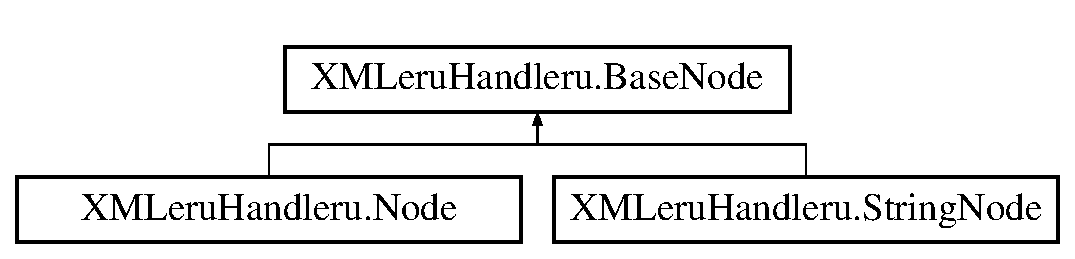
\includegraphics[height=2.000000cm]{class_x_m_leru_handleru_1_1_base_node}
\end{center}
\end{figure}
\subsection*{Public Member Functions}
\begin{DoxyCompactItemize}
\item 
\hypertarget{class_x_m_leru_handleru_1_1_base_node_a6fcb5194ad2113e93bc45c17d728a07a}{}abstract \hyperlink{class_x_m_leru_handleru_1_1_base_node}{Base\+Node} {\bfseries Add\+Node} (string name)\label{class_x_m_leru_handleru_1_1_base_node_a6fcb5194ad2113e93bc45c17d728a07a}

\item 
\hypertarget{class_x_m_leru_handleru_1_1_base_node_a0f28227f706da1e001e48d281513fce4}{}abstract \hyperlink{class_x_m_leru_handleru_1_1_base_node}{Base\+Node} {\bfseries Add\+String} (string s)\label{class_x_m_leru_handleru_1_1_base_node_a0f28227f706da1e001e48d281513fce4}

\item 
\hypertarget{class_x_m_leru_handleru_1_1_base_node_ad5d3ecd24e6f39daaa6010da7b457ef0}{}abstract \hyperlink{class_x_m_leru_handleru_1_1_base_node}{Base\+Node} {\bfseries Add\+Child} (\hyperlink{class_x_m_leru_handleru_1_1_base_node}{Base\+Node} n)\label{class_x_m_leru_handleru_1_1_base_node_ad5d3ecd24e6f39daaa6010da7b457ef0}

\item 
\hypertarget{class_x_m_leru_handleru_1_1_base_node_a6281b4132c69263e42f79f48d83f0ee0}{}abstract void {\bfseries Add\+Attr} (string k, string v)\label{class_x_m_leru_handleru_1_1_base_node_a6281b4132c69263e42f79f48d83f0ee0}

\item 
\hypertarget{class_x_m_leru_handleru_1_1_base_node_ab3370786a72aea288391e5975f55ce4e}{}abstract \hyperlink{class_x_m_leru_handleru_1_1_base_node}{Base\+Node} {\bfseries Get\+Child} (int i)\label{class_x_m_leru_handleru_1_1_base_node_ab3370786a72aea288391e5975f55ce4e}

\item 
\hypertarget{class_x_m_leru_handleru_1_1_base_node_acd7c21e09ca9c074c0e17036e8bf7c67}{}abstract int {\bfseries Get\+Child\+Count} ()\label{class_x_m_leru_handleru_1_1_base_node_acd7c21e09ca9c074c0e17036e8bf7c67}

\item 
\hypertarget{class_x_m_leru_handleru_1_1_base_node_a479e738c0d51104fee57a025649aa69f}{}abstract List$<$ \hyperlink{class_x_m_leru_handleru_1_1_base_node}{Base\+Node} $>$ {\bfseries Get\+Css\+Like} (string query)\label{class_x_m_leru_handleru_1_1_base_node_a479e738c0d51104fee57a025649aa69f}

\item 
\hypertarget{class_x_m_leru_handleru_1_1_base_node_af4ccbd830749f6567dcd46c3cee42b74}{}abstract string {\bfseries To\+Xml} (int indent=0)\label{class_x_m_leru_handleru_1_1_base_node_af4ccbd830749f6567dcd46c3cee42b74}

\item 
\hypertarget{class_x_m_leru_handleru_1_1_base_node_a349b1cd86da86931a5445ad81046d2f3}{}abstract string {\bfseries Get\+Attr} (string k)\label{class_x_m_leru_handleru_1_1_base_node_a349b1cd86da86931a5445ad81046d2f3}

\end{DoxyCompactItemize}
\subsection*{Properties}
\begin{DoxyCompactItemize}
\item 
\hypertarget{class_x_m_leru_handleru_1_1_base_node_ac3c3e0c083a9da350e5511163668ac81}{}\hyperlink{class_x_m_leru_handleru_1_1_base_node}{Base\+Node} \hyperlink{class_x_m_leru_handleru_1_1_base_node_ac3c3e0c083a9da350e5511163668ac81}{Parent}\hspace{0.3cm}{\ttfamily  \mbox{[}get, set\mbox{]}}\label{class_x_m_leru_handleru_1_1_base_node_ac3c3e0c083a9da350e5511163668ac81}

\begin{DoxyCompactList}\small\item\em The parent node. \end{DoxyCompactList}\item 
\hypertarget{class_x_m_leru_handleru_1_1_base_node_a693bfdbaf05b7554897d475afd2f4768}{}string \hyperlink{class_x_m_leru_handleru_1_1_base_node_a693bfdbaf05b7554897d475afd2f4768}{Name}\hspace{0.3cm}{\ttfamily  \mbox{[}get, protected set\mbox{]}}\label{class_x_m_leru_handleru_1_1_base_node_a693bfdbaf05b7554897d475afd2f4768}

\begin{DoxyCompactList}\small\item\em The name of the node. \end{DoxyCompactList}\end{DoxyCompactItemize}


\subsection{Detailed Description}
The abstract class that contains every method for the different nodes. 

The documentation for this class was generated from the following file\+:\begin{DoxyCompactItemize}
\item 
X\+M\+Leru\+Handleru/Base\+Node.\+cs\end{DoxyCompactItemize}

\hypertarget{class_x_m_leru_handleru_1_1_node}{}\section{X\+M\+Leru\+Handleru.\+Node Class Reference}
\label{class_x_m_leru_handleru_1_1_node}\index{X\+M\+Leru\+Handleru.\+Node@{X\+M\+Leru\+Handleru.\+Node}}
Inheritance diagram for X\+M\+Leru\+Handleru.\+Node\+:\begin{figure}[H]
\begin{center}
\leavevmode
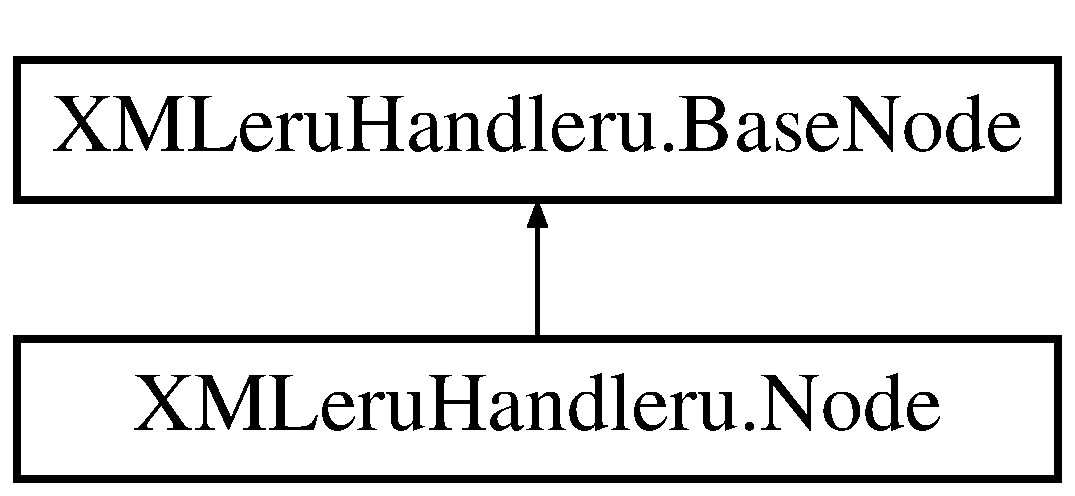
\includegraphics[height=2.000000cm]{class_x_m_leru_handleru_1_1_node}
\end{center}
\end{figure}
\subsection*{Public Member Functions}
\begin{DoxyCompactItemize}
\item 
\hyperlink{class_x_m_leru_handleru_1_1_node_af3e096333b8dcc74789ebc04c0984856}{Node} (string name, \hyperlink{class_x_m_leru_handleru_1_1_base_node}{Base\+Node} parent, Dictionary$<$ string, string $>$ attributes)
\begin{DoxyCompactList}\small\item\em Creates a new node without children. \end{DoxyCompactList}\item 
\hyperlink{class_x_m_leru_handleru_1_1_node_a8060ae6840e807ebf3d3ef7f27a468bf}{Node} (string name, \hyperlink{class_x_m_leru_handleru_1_1_base_node}{Base\+Node} parent)
\begin{DoxyCompactList}\small\item\em Creates a new node without children and attributes. \end{DoxyCompactList}\item 
\hyperlink{class_x_m_leru_handleru_1_1_node_ad8005a9ca54062189361e811e7064cff}{Node} (string name)
\begin{DoxyCompactList}\small\item\em Creates a new root node without children, attributes and parent. \end{DoxyCompactList}\item 
override \hyperlink{class_x_m_leru_handleru_1_1_base_node}{Base\+Node} \hyperlink{class_x_m_leru_handleru_1_1_node_aa79ab2740c301fca30270de273d1c796}{Add\+Node} (string name)
\begin{DoxyCompactList}\small\item\em Creates and adds a child \hyperlink{class_x_m_leru_handleru_1_1_node}{Node}. \end{DoxyCompactList}\item 
override \hyperlink{class_x_m_leru_handleru_1_1_base_node}{Base\+Node} \hyperlink{class_x_m_leru_handleru_1_1_node_ad6070ed490bfde070bdb07461fd873e1}{Add\+Child} (\hyperlink{class_x_m_leru_handleru_1_1_base_node}{Base\+Node} n)
\begin{DoxyCompactList}\small\item\em Adds a child. \end{DoxyCompactList}\item 
override \hyperlink{class_x_m_leru_handleru_1_1_base_node}{Base\+Node} \hyperlink{class_x_m_leru_handleru_1_1_node_a74b20c07c1d044392ae7670d58679c90}{Add\+String} (string s)
\begin{DoxyCompactList}\small\item\em Creates and adds a child \hyperlink{class_x_m_leru_handleru_1_1_string_node}{String\+Node}. \end{DoxyCompactList}\item 
override void \hyperlink{class_x_m_leru_handleru_1_1_node_af847932f7294cc39d8a3f6f89062a950}{Add\+Attr} (string k, string v)
\begin{DoxyCompactList}\small\item\em Adds an attribute. \end{DoxyCompactList}\item 
override string \hyperlink{class_x_m_leru_handleru_1_1_node_a29a231aa34d23b491600f13916bcb5de}{To\+Xml} (int indent=0)
\begin{DoxyCompactList}\small\item\em Creates an xml string. \end{DoxyCompactList}\item 
override string \hyperlink{class_x_m_leru_handleru_1_1_node_aa35d6d52814845f0c3f72ccdcdc20d13}{To\+String} ()
\begin{DoxyCompactList}\small\item\em Creates a string representation of the node. \end{DoxyCompactList}\item 
override \hyperlink{class_x_m_leru_handleru_1_1_base_node}{Base\+Node} \hyperlink{class_x_m_leru_handleru_1_1_node_a2e756780a13a8ce3f8b84aaa61a6c0cc}{Get\+Child} (int i)
\begin{DoxyCompactList}\small\item\em Returns the i\+:th child. \end{DoxyCompactList}\item 
override int \hyperlink{class_x_m_leru_handleru_1_1_node_a8d024d88abb37f16a7b46cb5bfdf5345}{Get\+Child\+Count} ()
\begin{DoxyCompactList}\small\item\em Returns the number of children. \end{DoxyCompactList}\item 
override List$<$ \hyperlink{class_x_m_leru_handleru_1_1_base_node}{Base\+Node} $>$ \hyperlink{class_x_m_leru_handleru_1_1_node_a2d2c1b582bd36ee9241763d108bd82e0}{Get\+Css\+Like} (string query)
\begin{DoxyCompactList}\small\item\em Not impelmented. \end{DoxyCompactList}\end{DoxyCompactItemize}
\subsection*{Properties}
\begin{DoxyCompactItemize}
\item 
\hypertarget{class_x_m_leru_handleru_1_1_node_afa682372142a202eca56962f9ca4eb6a}{}List$<$ \hyperlink{class_x_m_leru_handleru_1_1_base_node}{Base\+Node} $>$ {\bfseries Children}\hspace{0.3cm}{\ttfamily  \mbox{[}get, set\mbox{]}}\label{class_x_m_leru_handleru_1_1_node_afa682372142a202eca56962f9ca4eb6a}

\item 
\hypertarget{class_x_m_leru_handleru_1_1_node_a4d11bd34b693152c527f9add8997cea5}{}Dictionary$<$ string, string $>$ {\bfseries Attributes}\hspace{0.3cm}{\ttfamily  \mbox{[}get, set\mbox{]}}\label{class_x_m_leru_handleru_1_1_node_a4d11bd34b693152c527f9add8997cea5}

\end{DoxyCompactItemize}
\subsection*{Private Member Functions}
\begin{DoxyCompactItemize}
\item 
string \hyperlink{class_x_m_leru_handleru_1_1_node_aeb431cd29311f2a157930ae31cb61bf8}{Attributes\+To\+String} ()
\begin{DoxyCompactList}\small\item\em Converts the dictionary of attributes to a string. \end{DoxyCompactList}\end{DoxyCompactItemize}


\subsection{Constructor \& Destructor Documentation}
\hypertarget{class_x_m_leru_handleru_1_1_node_af3e096333b8dcc74789ebc04c0984856}{}\index{X\+M\+Leru\+Handleru\+::\+Node@{X\+M\+Leru\+Handleru\+::\+Node}!Node@{Node}}
\index{Node@{Node}!X\+M\+Leru\+Handleru\+::\+Node@{X\+M\+Leru\+Handleru\+::\+Node}}
\subsubsection[{Node}]{\setlength{\rightskip}{0pt plus 5cm}X\+M\+Leru\+Handleru.\+Node.\+Node (
\begin{DoxyParamCaption}
\item[{string}]{name, }
\item[{{\bf Base\+Node}}]{parent, }
\item[{Dictionary$<$ string, string $>$}]{attributes}
\end{DoxyParamCaption}
)\hspace{0.3cm}{\ttfamily [inline]}}\label{class_x_m_leru_handleru_1_1_node_af3e096333b8dcc74789ebc04c0984856}


Creates a new node without children. 


\begin{DoxyParams}{Parameters}
{\em name} & The name of the node \\
\hline
{\em parent} & The nodes parent or null if the node is root \\
\hline
{\em attributes} & The attributes associated with the node \\
\hline
\end{DoxyParams}
\hypertarget{class_x_m_leru_handleru_1_1_node_a8060ae6840e807ebf3d3ef7f27a468bf}{}\index{X\+M\+Leru\+Handleru\+::\+Node@{X\+M\+Leru\+Handleru\+::\+Node}!Node@{Node}}
\index{Node@{Node}!X\+M\+Leru\+Handleru\+::\+Node@{X\+M\+Leru\+Handleru\+::\+Node}}
\subsubsection[{Node}]{\setlength{\rightskip}{0pt plus 5cm}X\+M\+Leru\+Handleru.\+Node.\+Node (
\begin{DoxyParamCaption}
\item[{string}]{name, }
\item[{{\bf Base\+Node}}]{parent}
\end{DoxyParamCaption}
)\hspace{0.3cm}{\ttfamily [inline]}}\label{class_x_m_leru_handleru_1_1_node_a8060ae6840e807ebf3d3ef7f27a468bf}


Creates a new node without children and attributes. 


\begin{DoxyParams}{Parameters}
{\em name} & The name of the node \\
\hline
{\em parent} & The nodes parent or null if the node is root \\
\hline
\end{DoxyParams}
\hypertarget{class_x_m_leru_handleru_1_1_node_ad8005a9ca54062189361e811e7064cff}{}\index{X\+M\+Leru\+Handleru\+::\+Node@{X\+M\+Leru\+Handleru\+::\+Node}!Node@{Node}}
\index{Node@{Node}!X\+M\+Leru\+Handleru\+::\+Node@{X\+M\+Leru\+Handleru\+::\+Node}}
\subsubsection[{Node}]{\setlength{\rightskip}{0pt plus 5cm}X\+M\+Leru\+Handleru.\+Node.\+Node (
\begin{DoxyParamCaption}
\item[{string}]{name}
\end{DoxyParamCaption}
)\hspace{0.3cm}{\ttfamily [inline]}}\label{class_x_m_leru_handleru_1_1_node_ad8005a9ca54062189361e811e7064cff}


Creates a new root node without children, attributes and parent. 


\begin{DoxyParams}{Parameters}
{\em name} & The name of the node \\
\hline
\end{DoxyParams}


\subsection{Member Function Documentation}
\hypertarget{class_x_m_leru_handleru_1_1_node_af847932f7294cc39d8a3f6f89062a950}{}\index{X\+M\+Leru\+Handleru\+::\+Node@{X\+M\+Leru\+Handleru\+::\+Node}!Add\+Attr@{Add\+Attr}}
\index{Add\+Attr@{Add\+Attr}!X\+M\+Leru\+Handleru\+::\+Node@{X\+M\+Leru\+Handleru\+::\+Node}}
\subsubsection[{Add\+Attr}]{\setlength{\rightskip}{0pt plus 5cm}override void X\+M\+Leru\+Handleru.\+Node.\+Add\+Attr (
\begin{DoxyParamCaption}
\item[{string}]{k, }
\item[{string}]{v}
\end{DoxyParamCaption}
)\hspace{0.3cm}{\ttfamily [inline]}, {\ttfamily [virtual]}}\label{class_x_m_leru_handleru_1_1_node_af847932f7294cc39d8a3f6f89062a950}


Adds an attribute. 


\begin{DoxyParams}{Parameters}
{\em k} & The attribute key \\
\hline
{\em v} & The attribute value \\
\hline
\end{DoxyParams}
\begin{DoxyReturn}{Returns}
void 
\end{DoxyReturn}


Implements \hyperlink{class_x_m_leru_handleru_1_1_base_node}{X\+M\+Leru\+Handleru.\+Base\+Node}.

\hypertarget{class_x_m_leru_handleru_1_1_node_ad6070ed490bfde070bdb07461fd873e1}{}\index{X\+M\+Leru\+Handleru\+::\+Node@{X\+M\+Leru\+Handleru\+::\+Node}!Add\+Child@{Add\+Child}}
\index{Add\+Child@{Add\+Child}!X\+M\+Leru\+Handleru\+::\+Node@{X\+M\+Leru\+Handleru\+::\+Node}}
\subsubsection[{Add\+Child}]{\setlength{\rightskip}{0pt plus 5cm}override {\bf Base\+Node} X\+M\+Leru\+Handleru.\+Node.\+Add\+Child (
\begin{DoxyParamCaption}
\item[{{\bf Base\+Node}}]{n}
\end{DoxyParamCaption}
)\hspace{0.3cm}{\ttfamily [inline]}, {\ttfamily [virtual]}}\label{class_x_m_leru_handleru_1_1_node_ad6070ed490bfde070bdb07461fd873e1}


Adds a child. 


\begin{DoxyParams}{Parameters}
{\em n} & The child to add \\
\hline
\end{DoxyParams}
\begin{DoxyReturn}{Returns}
The added child 
\end{DoxyReturn}


Implements \hyperlink{class_x_m_leru_handleru_1_1_base_node}{X\+M\+Leru\+Handleru.\+Base\+Node}.

\hypertarget{class_x_m_leru_handleru_1_1_node_aa79ab2740c301fca30270de273d1c796}{}\index{X\+M\+Leru\+Handleru\+::\+Node@{X\+M\+Leru\+Handleru\+::\+Node}!Add\+Node@{Add\+Node}}
\index{Add\+Node@{Add\+Node}!X\+M\+Leru\+Handleru\+::\+Node@{X\+M\+Leru\+Handleru\+::\+Node}}
\subsubsection[{Add\+Node}]{\setlength{\rightskip}{0pt plus 5cm}override {\bf Base\+Node} X\+M\+Leru\+Handleru.\+Node.\+Add\+Node (
\begin{DoxyParamCaption}
\item[{string}]{name}
\end{DoxyParamCaption}
)\hspace{0.3cm}{\ttfamily [inline]}, {\ttfamily [virtual]}}\label{class_x_m_leru_handleru_1_1_node_aa79ab2740c301fca30270de273d1c796}


Creates and adds a child \hyperlink{class_x_m_leru_handleru_1_1_node}{Node}. 


\begin{DoxyParams}{Parameters}
{\em name} & The name of the to be node \\
\hline
\end{DoxyParams}
\begin{DoxyReturn}{Returns}
The created node 
\end{DoxyReturn}


Implements \hyperlink{class_x_m_leru_handleru_1_1_base_node}{X\+M\+Leru\+Handleru.\+Base\+Node}.

\hypertarget{class_x_m_leru_handleru_1_1_node_a74b20c07c1d044392ae7670d58679c90}{}\index{X\+M\+Leru\+Handleru\+::\+Node@{X\+M\+Leru\+Handleru\+::\+Node}!Add\+String@{Add\+String}}
\index{Add\+String@{Add\+String}!X\+M\+Leru\+Handleru\+::\+Node@{X\+M\+Leru\+Handleru\+::\+Node}}
\subsubsection[{Add\+String}]{\setlength{\rightskip}{0pt plus 5cm}override {\bf Base\+Node} X\+M\+Leru\+Handleru.\+Node.\+Add\+String (
\begin{DoxyParamCaption}
\item[{string}]{s}
\end{DoxyParamCaption}
)\hspace{0.3cm}{\ttfamily [inline]}, {\ttfamily [virtual]}}\label{class_x_m_leru_handleru_1_1_node_a74b20c07c1d044392ae7670d58679c90}


Creates and adds a child \hyperlink{class_x_m_leru_handleru_1_1_string_node}{String\+Node}. 


\begin{DoxyParams}{Parameters}
{\em s} & The content of the to be node \\
\hline
\end{DoxyParams}
\begin{DoxyReturn}{Returns}
The created node 
\end{DoxyReturn}


Implements \hyperlink{class_x_m_leru_handleru_1_1_base_node}{X\+M\+Leru\+Handleru.\+Base\+Node}.

\hypertarget{class_x_m_leru_handleru_1_1_node_aeb431cd29311f2a157930ae31cb61bf8}{}\index{X\+M\+Leru\+Handleru\+::\+Node@{X\+M\+Leru\+Handleru\+::\+Node}!Attributes\+To\+String@{Attributes\+To\+String}}
\index{Attributes\+To\+String@{Attributes\+To\+String}!X\+M\+Leru\+Handleru\+::\+Node@{X\+M\+Leru\+Handleru\+::\+Node}}
\subsubsection[{Attributes\+To\+String}]{\setlength{\rightskip}{0pt plus 5cm}string X\+M\+Leru\+Handleru.\+Node.\+Attributes\+To\+String (
\begin{DoxyParamCaption}
{}
\end{DoxyParamCaption}
)\hspace{0.3cm}{\ttfamily [inline]}, {\ttfamily [private]}}\label{class_x_m_leru_handleru_1_1_node_aeb431cd29311f2a157930ae31cb61bf8}


Converts the dictionary of attributes to a string. 

\begin{DoxyReturn}{Returns}
The string 
\end{DoxyReturn}
\hypertarget{class_x_m_leru_handleru_1_1_node_a2e756780a13a8ce3f8b84aaa61a6c0cc}{}\index{X\+M\+Leru\+Handleru\+::\+Node@{X\+M\+Leru\+Handleru\+::\+Node}!Get\+Child@{Get\+Child}}
\index{Get\+Child@{Get\+Child}!X\+M\+Leru\+Handleru\+::\+Node@{X\+M\+Leru\+Handleru\+::\+Node}}
\subsubsection[{Get\+Child}]{\setlength{\rightskip}{0pt plus 5cm}override {\bf Base\+Node} X\+M\+Leru\+Handleru.\+Node.\+Get\+Child (
\begin{DoxyParamCaption}
\item[{int}]{i}
\end{DoxyParamCaption}
)\hspace{0.3cm}{\ttfamily [inline]}, {\ttfamily [virtual]}}\label{class_x_m_leru_handleru_1_1_node_a2e756780a13a8ce3f8b84aaa61a6c0cc}


Returns the i\+:th child. 


\begin{DoxyParams}{Parameters}
{\em i} & The index of child to get from \\
\hline
\end{DoxyParams}
\begin{DoxyReturn}{Returns}
The child 
\end{DoxyReturn}


Implements \hyperlink{class_x_m_leru_handleru_1_1_base_node}{X\+M\+Leru\+Handleru.\+Base\+Node}.

\hypertarget{class_x_m_leru_handleru_1_1_node_a8d024d88abb37f16a7b46cb5bfdf5345}{}\index{X\+M\+Leru\+Handleru\+::\+Node@{X\+M\+Leru\+Handleru\+::\+Node}!Get\+Child\+Count@{Get\+Child\+Count}}
\index{Get\+Child\+Count@{Get\+Child\+Count}!X\+M\+Leru\+Handleru\+::\+Node@{X\+M\+Leru\+Handleru\+::\+Node}}
\subsubsection[{Get\+Child\+Count}]{\setlength{\rightskip}{0pt plus 5cm}override int X\+M\+Leru\+Handleru.\+Node.\+Get\+Child\+Count (
\begin{DoxyParamCaption}
{}
\end{DoxyParamCaption}
)\hspace{0.3cm}{\ttfamily [inline]}, {\ttfamily [virtual]}}\label{class_x_m_leru_handleru_1_1_node_a8d024d88abb37f16a7b46cb5bfdf5345}


Returns the number of children. 

\begin{DoxyReturn}{Returns}
The number of childre 
\end{DoxyReturn}


Implements \hyperlink{class_x_m_leru_handleru_1_1_base_node}{X\+M\+Leru\+Handleru.\+Base\+Node}.

\hypertarget{class_x_m_leru_handleru_1_1_node_a2d2c1b582bd36ee9241763d108bd82e0}{}\index{X\+M\+Leru\+Handleru\+::\+Node@{X\+M\+Leru\+Handleru\+::\+Node}!Get\+Css\+Like@{Get\+Css\+Like}}
\index{Get\+Css\+Like@{Get\+Css\+Like}!X\+M\+Leru\+Handleru\+::\+Node@{X\+M\+Leru\+Handleru\+::\+Node}}
\subsubsection[{Get\+Css\+Like}]{\setlength{\rightskip}{0pt plus 5cm}override List$<${\bf Base\+Node}$>$ X\+M\+Leru\+Handleru.\+Node.\+Get\+Css\+Like (
\begin{DoxyParamCaption}
\item[{string}]{query}
\end{DoxyParamCaption}
)\hspace{0.3cm}{\ttfamily [inline]}, {\ttfamily [virtual]}}\label{class_x_m_leru_handleru_1_1_node_a2d2c1b582bd36ee9241763d108bd82e0}


Not impelmented. 


\begin{DoxyParams}{Parameters}
{\em query} & The query \\
\hline
\end{DoxyParams}
\begin{DoxyReturn}{Returns}
A list of the matching nodes 
\end{DoxyReturn}


Implements \hyperlink{class_x_m_leru_handleru_1_1_base_node}{X\+M\+Leru\+Handleru.\+Base\+Node}.

\hypertarget{class_x_m_leru_handleru_1_1_node_aa35d6d52814845f0c3f72ccdcdc20d13}{}\index{X\+M\+Leru\+Handleru\+::\+Node@{X\+M\+Leru\+Handleru\+::\+Node}!To\+String@{To\+String}}
\index{To\+String@{To\+String}!X\+M\+Leru\+Handleru\+::\+Node@{X\+M\+Leru\+Handleru\+::\+Node}}
\subsubsection[{To\+String}]{\setlength{\rightskip}{0pt plus 5cm}override string X\+M\+Leru\+Handleru.\+Node.\+To\+String (
\begin{DoxyParamCaption}
{}
\end{DoxyParamCaption}
)\hspace{0.3cm}{\ttfamily [inline]}}\label{class_x_m_leru_handleru_1_1_node_aa35d6d52814845f0c3f72ccdcdc20d13}


Creates a string representation of the node. 

\begin{DoxyReturn}{Returns}
The corresponding xml string 
\end{DoxyReturn}
\hypertarget{class_x_m_leru_handleru_1_1_node_a29a231aa34d23b491600f13916bcb5de}{}\index{X\+M\+Leru\+Handleru\+::\+Node@{X\+M\+Leru\+Handleru\+::\+Node}!To\+Xml@{To\+Xml}}
\index{To\+Xml@{To\+Xml}!X\+M\+Leru\+Handleru\+::\+Node@{X\+M\+Leru\+Handleru\+::\+Node}}
\subsubsection[{To\+Xml}]{\setlength{\rightskip}{0pt plus 5cm}override string X\+M\+Leru\+Handleru.\+Node.\+To\+Xml (
\begin{DoxyParamCaption}
\item[{int}]{indent = {\ttfamily 0}}
\end{DoxyParamCaption}
)\hspace{0.3cm}{\ttfamily [inline]}, {\ttfamily [virtual]}}\label{class_x_m_leru_handleru_1_1_node_a29a231aa34d23b491600f13916bcb5de}


Creates an xml string. 


\begin{DoxyParams}{Parameters}
{\em indent} & the number of spaces indentation for current indentation level \\
\hline
\end{DoxyParams}
\begin{DoxyReturn}{Returns}
The xml string 
\end{DoxyReturn}


Implements \hyperlink{class_x_m_leru_handleru_1_1_base_node}{X\+M\+Leru\+Handleru.\+Base\+Node}.



The documentation for this class was generated from the following file\+:\begin{DoxyCompactItemize}
\item 
X\+M\+Leru\+Handleru/Node.\+cs\end{DoxyCompactItemize}

\hypertarget{class_x_m_leru_handleru_1_1_program}{}\section{X\+M\+Leru\+Handleru.\+Program Class Reference}
\label{class_x_m_leru_handleru_1_1_program}\index{X\+M\+Leru\+Handleru.\+Program@{X\+M\+Leru\+Handleru.\+Program}}
\subsection*{Static Public Member Functions}
\begin{DoxyCompactItemize}
\item 
\hypertarget{class_x_m_leru_handleru_1_1_program_a1fac06cc0ab95a39af3c262ae2152739}{}static void {\bfseries Test\+Manual\+Create\+And\+Print} ()\label{class_x_m_leru_handleru_1_1_program_a1fac06cc0ab95a39af3c262ae2152739}

\item 
\hypertarget{class_x_m_leru_handleru_1_1_program_a46277b5cc2e1f90abc6072dbf7b3bd28}{}static void {\bfseries Test\+Load\+And\+Print\+X\+M\+L} ()\label{class_x_m_leru_handleru_1_1_program_a46277b5cc2e1f90abc6072dbf7b3bd28}

\item 
\hypertarget{class_x_m_leru_handleru_1_1_program_a928ffe04f368b42de64fd208a2b2548d}{}static void {\bfseries Test\+Load\+And\+Save\+To\+File} ()\label{class_x_m_leru_handleru_1_1_program_a928ffe04f368b42de64fd208a2b2548d}

\end{DoxyCompactItemize}
\subsection*{Static Private Member Functions}
\begin{DoxyCompactItemize}
\item 
\hypertarget{class_x_m_leru_handleru_1_1_program_a6d7fc302b636f572052e0fe0b63307d6}{}static void {\bfseries Main} (string\mbox{[}$\,$\mbox{]} args)\label{class_x_m_leru_handleru_1_1_program_a6d7fc302b636f572052e0fe0b63307d6}

\end{DoxyCompactItemize}


The documentation for this class was generated from the following file\+:\begin{DoxyCompactItemize}
\item 
X\+M\+Leru\+Handleru/Program.\+cs\end{DoxyCompactItemize}

\hypertarget{class_x_m_leru_handleru_1_1_string_node}{}\section{X\+M\+Leru\+Handleru.\+String\+Node Class Reference}
\label{class_x_m_leru_handleru_1_1_string_node}\index{X\+M\+Leru\+Handleru.\+String\+Node@{X\+M\+Leru\+Handleru.\+String\+Node}}
Inheritance diagram for X\+M\+Leru\+Handleru.\+String\+Node\+:\begin{figure}[H]
\begin{center}
\leavevmode
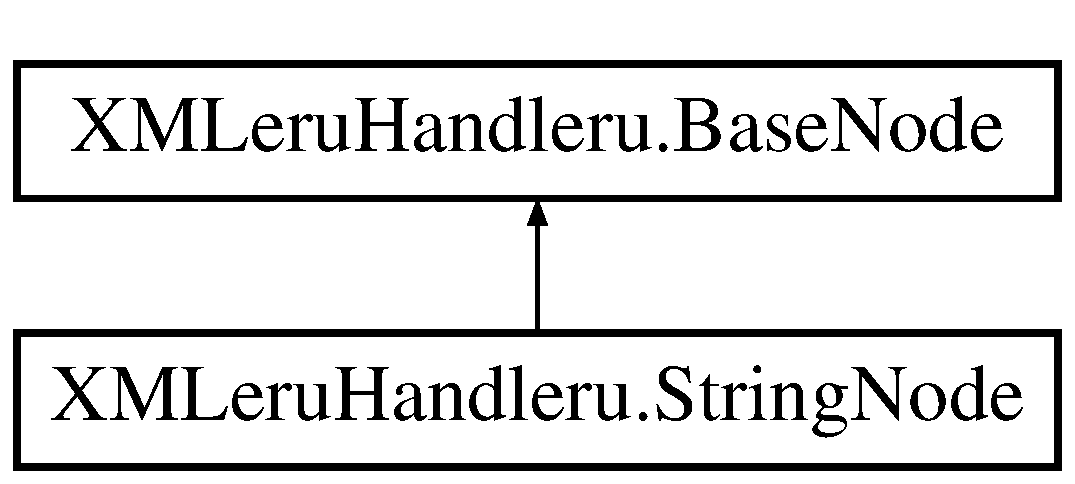
\includegraphics[height=2.000000cm]{class_x_m_leru_handleru_1_1_string_node}
\end{center}
\end{figure}
\subsection*{Public Member Functions}
\begin{DoxyCompactItemize}
\item 
\hypertarget{class_x_m_leru_handleru_1_1_string_node_a4c1eafc0ac995e89ef5a4af85c0f9c19}{}{\bfseries String\+Node} (string name, \hyperlink{class_x_m_leru_handleru_1_1_base_node}{Base\+Node} parent)\label{class_x_m_leru_handleru_1_1_string_node_a4c1eafc0ac995e89ef5a4af85c0f9c19}

\item 
\hypertarget{class_x_m_leru_handleru_1_1_string_node_a577acb87d6791fc9aeacaf9e8e6effcb}{}override \hyperlink{class_x_m_leru_handleru_1_1_base_node}{Base\+Node} {\bfseries Add\+Node} (string name)\label{class_x_m_leru_handleru_1_1_string_node_a577acb87d6791fc9aeacaf9e8e6effcb}

\item 
\hypertarget{class_x_m_leru_handleru_1_1_string_node_a4e5019cd4fa98a233d1d1d580a861dc4}{}override \hyperlink{class_x_m_leru_handleru_1_1_base_node}{Base\+Node} {\bfseries Add\+Child} (\hyperlink{class_x_m_leru_handleru_1_1_base_node}{Base\+Node} n)\label{class_x_m_leru_handleru_1_1_string_node_a4e5019cd4fa98a233d1d1d580a861dc4}

\item 
\hypertarget{class_x_m_leru_handleru_1_1_string_node_a5eb5f6d350d6fe0561e9bee5370f9038}{}override \hyperlink{class_x_m_leru_handleru_1_1_base_node}{Base\+Node} {\bfseries Add\+String} (string s)\label{class_x_m_leru_handleru_1_1_string_node_a5eb5f6d350d6fe0561e9bee5370f9038}

\item 
\hypertarget{class_x_m_leru_handleru_1_1_string_node_ad90914dceb59dd26271f5266b2d899ca}{}override void {\bfseries Add\+Attr} (string k, string v)\label{class_x_m_leru_handleru_1_1_string_node_ad90914dceb59dd26271f5266b2d899ca}

\item 
\hypertarget{class_x_m_leru_handleru_1_1_string_node_aeefff8d4054ec20dc817b7cda8130cd6}{}override string {\bfseries To\+String} ()\label{class_x_m_leru_handleru_1_1_string_node_aeefff8d4054ec20dc817b7cda8130cd6}

\item 
\hypertarget{class_x_m_leru_handleru_1_1_string_node_ac8507d872f9ad6789758b080894ad78f}{}override string {\bfseries To\+Xml} (int indent=0)\label{class_x_m_leru_handleru_1_1_string_node_ac8507d872f9ad6789758b080894ad78f}

\item 
\hypertarget{class_x_m_leru_handleru_1_1_string_node_aab1723e0d3ece1da14a5e3ebf07bf541}{}override \hyperlink{class_x_m_leru_handleru_1_1_base_node}{Base\+Node} {\bfseries get\+Child} (int i)\label{class_x_m_leru_handleru_1_1_string_node_aab1723e0d3ece1da14a5e3ebf07bf541}

\item 
\hypertarget{class_x_m_leru_handleru_1_1_string_node_a2207b714636aa065f607108d19994757}{}override int {\bfseries get\+Child\+Count} ()\label{class_x_m_leru_handleru_1_1_string_node_a2207b714636aa065f607108d19994757}

\item 
\hypertarget{class_x_m_leru_handleru_1_1_string_node_af1a0f24fafb8da6a57e72c951bb16dc1}{}override List$<$ \hyperlink{class_x_m_leru_handleru_1_1_base_node}{Base\+Node} $>$ {\bfseries Get\+Css\+Like} (string xpath)\label{class_x_m_leru_handleru_1_1_string_node_af1a0f24fafb8da6a57e72c951bb16dc1}

\end{DoxyCompactItemize}
\subsection*{Additional Inherited Members}


The documentation for this class was generated from the following file\+:\begin{DoxyCompactItemize}
\item 
X\+M\+Leru\+Handleru/String\+Node.\+cs\end{DoxyCompactItemize}

\hypertarget{class_x_m_leru_handleru_1_1_x_m_l_file_manager}{}\section{X\+M\+Leru\+Handleru.\+X\+M\+L\+File\+Manager Class Reference}
\label{class_x_m_leru_handleru_1_1_x_m_l_file_manager}\index{X\+M\+Leru\+Handleru.\+X\+M\+L\+File\+Manager@{X\+M\+Leru\+Handleru.\+X\+M\+L\+File\+Manager}}
\subsection*{Static Public Member Functions}
\begin{DoxyCompactItemize}
\item 
\hypertarget{class_x_m_leru_handleru_1_1_x_m_l_file_manager_af518835562c9dc0e93f2f737923a0935}{}static void {\bfseries Save\+To\+File} (string path, \hyperlink{class_x_m_leru_handleru_1_1_base_node}{Base\+Node} node)\label{class_x_m_leru_handleru_1_1_x_m_l_file_manager_af518835562c9dc0e93f2f737923a0935}

\item 
\hypertarget{class_x_m_leru_handleru_1_1_x_m_l_file_manager_a2e3dfed69563014bb11b61699ce76799}{}static \hyperlink{class_x_m_leru_handleru_1_1_base_node}{Base\+Node} {\bfseries Load\+File} (string path)\label{class_x_m_leru_handleru_1_1_x_m_l_file_manager_a2e3dfed69563014bb11b61699ce76799}

\item 
\hypertarget{class_x_m_leru_handleru_1_1_x_m_l_file_manager_af04699e6a4e0195b2e408e52aab1eaee}{}static \hyperlink{class_x_m_leru_handleru_1_1_base_node}{Base\+Node} {\bfseries Load\+String} (string xml)\label{class_x_m_leru_handleru_1_1_x_m_l_file_manager_af04699e6a4e0195b2e408e52aab1eaee}

\end{DoxyCompactItemize}


The documentation for this class was generated from the following file\+:\begin{DoxyCompactItemize}
\item 
X\+M\+Leru\+Handleru/X\+M\+L\+File\+Manager.\+cs\end{DoxyCompactItemize}

%--- End generated contents ---

% Index
\backmatter
\newpage
\phantomsection
\clearemptydoublepage
\addcontentsline{toc}{chapter}{Index}
\printindex

\end{document}
